\section{Linear Classifiers}
\label{sec:Linear Classifiers}
It is reasonable to start with two of the most intuitive and famous methods for classification, LDA and Logistic Regression. The point of the following chapters is to give a general introduction to some methods for classification, and therefore only two classes will be considered. Later this framework will be expanded to include multiple classes.
%
\subsection{LDA and Fisher's linear discriminant}
\label{sub:LDA and Fisher's linear discriminant}
This section should be considered a summary from \cite[ch.~4.1.4]{bishop} and \cite[ch.~4.3]{modstat}, and no further references to these books will be made. \\
\\
The idea in Fisher's linear discriminant is to find a discriminant hyperplane in the features $\mathbf{x}\in \mathbb{R}^D$. This is done by finding a vector $\mathbf{w}$, that the features are projected on and thus reducing the problem to one dimension in 
\begin{align}
  z = \mathbf{w}'\mathbf{x}.
\end{align}
If $\mathbf{w}$ is chosen well, one can find a threshold $t$, and classify to class $\mathcal{C}_1$ if $z > t$ and to class $\mathcal{C}_2$ if not. The problem is therefore, how to find the vector $\mathbf{w}$ that gives the best class separation. One approach is to let $\mathbf{w}$ be proportional to the vector between the class means, i.e. $\mathbf{w} \propto (\bm{\mu}_2 - \bm{\mu}_1)$, where $\bm{\mu}_k = \sum_{i \in \mathcal{C}_k} \mathbf{x}_i/N_k$, and $N_k$ is the number of training points in $\mathcal{C}_k$. However, this does not take into account the orientation of the points around the mean. This causes problems if the variance is high in some direction perpendicular to $(\bm{\mu}_2 - \bm{\mu}_1)$. Fisher's approach is to also take this within-class variance into account, by minimize it on the projected line. So he want the $\mathbf{w}$ that maximize the between-class variance $(\mu_2 - \mu_1)^2$ and minimize the within-class variance $s_1^2 + s_2^2$. 
\begin{align}
  \label{eq:fisherMax} 
  \mathbf{w} &= \argmax_{\mathbf{v}} \frac{(\mu_2 - \mu_1)^2}{s_1^2 + s_2^2} \\
  s_k^2 &= \sum_{i \in \mathcal{C}_k} (z_i - m_k)^2, \quad \mu_k = \mathbf{v}'\bm{\mu}_k.
\end{align}
Now let 
\begin{align}
  \mathbf{S}_W &= \mathbf{S}_1 + \mathbf{S}_2, \quad  \mathbf{S}_k =  \sum_{i \in \mathcal{C}_k} (\mathbf{x}_i - \bm{\mu}_k)(\mathbf{x}_i - \bm{\mu}_k)', \\
  \label{eq:SB} 
  \mathbf{S}_B &= (\bm{\mu}_2 - \bm{\mu}_1)(\bm{\mu}_2 - \bm{\mu}_1)'
\end{align}
\colorbox{yellow}{1/(N-1) differs in wikipedia and bishop}\\
denote the total within- and between-class covariances, and \eqref{eq:fisherMax} can be written as
\\ \colorbox{yellow}{Not 1/N means we weight covariances by nr of points}\\
\begin{align}
  \mathbf{w} = \argmax_v  \frac{\mathbf{v}'\mathbf{S}_B \mathbf{v}}{\mathbf{v}' \mathbf{S}_W \mathbf{v}}.
\end{align}
By differentiating and setting the expression equal to zero one get
\begin{align}
  (\mathbf{w}' \mathbf{S}_B \mathbf{w})\mathbf{S}_W \mathbf{w} = (\mathbf{w}' \mathbf{S}_W \mathbf{w})\mathbf{S}_B \mathbf{w}.
\end{align}
From \eqref{eq:SB}, it follows that that $(\bm{\mu}_2 - \bm{\mu}_1)$ is proportional to $\mathbf{S}_B \mathbf{v}$. This yields Fisher's linear discriminant
\begin{align}
  \mathbf{w} \propto \mathbf{S}_W^{-1} (\bm \mu_2 - \bm \mu_1).
\end{align}
Note that even the terms \textit{variance} and \textit{covariance} are used, the expressions are not averaged. This is just to simplify notation. \\
\\
The term Linear discriminant analysis, or LDA, and Fisher's linear discriminant are often used interchangeably. Only the derivation differs. For LDA it takes a Bayesian approach. Assume the prior distribution of the classes $Y=k$, $\pi_k$, and the conditional distribution of $X$ given $Y$, $f_k(\mathbf{x})$ are known. Simple application of the Bayes theorem yields 
\begin{align}
  P(Y=k|X=\mathbf{x}) = \frac{f_k(\mathbf{x}) \pi_k}{\sum^{K}_{i=1} f_i(\mathbf{x})\pi_i} .
\end{align}
Using this posterior distribution to create
\begin{align}
  \label{eq:bayesian} 
  C(\mathbf{x}) = \argmax_k P(Y=k|X=\mathbf{x}),
\end{align}
which is called the \textit{Bayes classifier} \cite[p.~21]{modstat}. It is clear that this is the best one can do, and the Bayes classifier is therefor often used as a benchmark in simulation studies. As the prior and conditional distribution are not know, there are numerous approaches use different assumptions on these. LDA assume the conditional distributions are multivariate Gaussian with same covariance $\bm{\Sigma}$ and different mean $\bm\mu_k$
\begin{align}
  f_k(\mathbf{x}) =  \frac{1}{(2\pi)^{N_k/2}|\bm{\Sigma}|^{1/2}} \exp\left( -\frac{1}{2} (\mathbf{x}-\bm \mu_k)' \bm{\Sigma}^{-1} (\mathbf{x}-\bm \mu_k)\right).
\end{align}
The classifier is constructed by evaluating the log-ratio of the probabilities
\begin{align}
  \label{eq:lda} 
  \log{\frac{P(Y=2|X=\mathbf{x})}{P(Y=1|X=\mathbf{x})}} &= \log{\frac{f_2(\mathbf{x})}{f_1(\mathbf{x})} } + \log{\frac{\pi_2}{\pi_1} } \notag \ \\
  &= \log{\frac{\pi_2}{\pi_1}} -\frac{1}{2} (\bm \mu_2+\bm \mu_1)' \bm{\Sigma}^{-1} (\bm \mu_2-\bm \mu_1) \\
  & \quad + \mathbf{x}'\bm{\Sigma}^{-1} (\bm \mu_2-\bm \mu_1).
  \notag \ 
\end{align}
So one classify to $\mathcal{C}_2$ if \eqref{eq:lda} is positive and to $\mathcal{C}_1$ if not. Another approach is to use the only last part of \eqref{eq:lda}, $\mathbf{x}'\bm{\Sigma}^{-1} (\bm \mu_1-\bm \mu_2)$, and classify based on some threshold $t$ found by e.g. cross-validation. The reasoning behind this is that if the Gaussian assumptions are wrong, a better threshold can be created based on the training data. \\
\\
When using LDA, the parameters are not know, so they are usually estimated from the training data by
\begin{align}
   \hat{\pi}_k &= \frac{N_k}{N},  \\
   \hat{\bm \mu}_k &= \frac{1}{N_k} \sum_{i \in \mathcal{C}_k}\mathbf{x}_i, \\
   \hat{\bm \Sigma} &= \frac{1}{N-2} \sum_{k = 1}^{2} \sum_{i \in \mathcal{C}_k}(\mathbf{x}_i - \hat{\bm{\mu}}_k)(\mathbf{x}_i - \hat{\bm{\mu}}_k)'.
\end{align}
It now becomes clear that both LDA and Fisher's linear discriminant do the same projection. The only difference between the methods is that because of the Gaussian assumptions LDA can give a suggested threshold.
%
\subsection{Logistic Regression}
\label{sub:Logistic Regression}
\colorbox{yellow}{Optimization algorithms for finding parameters?}\\
The goal of logistic regression is to model the posterior class-probabilities and create a classifier based on them. As the probabilities should sum to one, it is obvious that they can not be linear in $\mathbf{x}$. The approach is therefore to assume the log-odds are linear in $\mathbf{x}$. 
\begin{align}
  \label{eq:logclass} 
   \log \frac{P(Y=2|X=\mathbf{x})}{P(Y=1|X=\mathbf{x})} = \beta_0 + \mathbf{x}'\bm \beta.
\end{align}
From now on it is assumed that $\beta_0 + \mathbf{x}' \bm \beta$ is written as $\mathbf{x}' \bm \beta$.
The function
\begin{align}
  logit(p_{ki}) = \log  \frac{p_{ki}}{1-p_{ki}},
\end{align}
where $p_{ki} = P(Y=k|X=\mathbf{x_i})$, is called \textit{the logit function} or \textit{link}. By inverting the logit function it becomes clear that the posterior probabilities sum to \textit{one}.
\begin{align}
  p_{2i} &=  \frac{e^{\mathbf{x}_i'\bm \beta}}{1 + e^{\mathbf{x}_i'\bm \beta}} \\
  p_{1i} &=  \frac{1}{1 + e^{\mathbf{x}_i'\bm \beta}}.
\end{align}
There are other choices than the logit function, e.g. the probit function based on Gaussian assumptions, however, they will not be covered in this paper. 
\todo{Refer to paper?}
Often there is little knowledge about the posterior distribution, so the logit might be as good a choice as any other. 
\todo{Remove this?}
To find good values for $\bm \beta$, it is common to use the MLE (Maximum likelihood estimator). Let $n_i$ be the number of training samples in gourp $i$ (common $\mathbf{x}_i$), and let $Z_i$ the amount in group $i$ that has class $2$. This means $Z_i$ is binomial distributed with
\begin{align}
  P(Z_i = z_i) = \binom{n_i}{z_i} p_{2i}^{z_i} (1-p_{2i})^{n_i - z_i}.
\end{align}
So the likelihood and log-likelihood are
\begin{align}
  L(\beta) &= \prod_{i = 1}^{N} P(Z_i = z_i). \\
  l(\beta) &\propto \sum^{N}_{i=1} z_i \log p_{2i} + (n_i - z_i) \log (1- p_{2i}).
\end{align}
There is no analytical solution that maximizes the likelihood, so one has to use a numerical optimization algorithm to find the MLE.  \todo{Elaborate optimization?}
After $\bm \beta$ is found, one can create a classifier the same way as for logistic regression, i.e. classify to $\mathcal{C}_2$ if \eqref{eq:logclass} is positive and to $\mathcal{C}_1$ if not. However, this assumes the logit link gives accurate probabilities. Often the choice of logit link is based on lack of a better choice so there is little suggesting the probabilities are particularly accurate. It might therefore be better to classify based on a threshold found by e.g. cross-validation. 
\\\colorbox{yellow}{Have hear a lot that logit is used because: "Why not".}
%
\subsection{LDA and Logistic Regression}
\label{sub:LDA and Logistic Regre}
<<ldaVsLogistic, echo = FALSE>>=
source("../code/ldaVsLogistic.R")
@
Comparing LDA and logistic regression, it is clear that they are both linear in the log odds. Obviously this does not restrict the decision boundary to be linear in $x_1, x_2, \ldots , x_D$. One can easily let $\mathbf{x}$ contain polynomial terms and interaction terms, like $(x_1, x_2, x_1^2, x_1 x_2, \ldots )$. This way one see that the decision boundary can be pretty flexible. Both methods are also easy to generalize to multi class classifiers, but this will not be done in this project. \todo{LDA categorical variables}\\
\\
To compare the two methods performance a toy example was generated by drawing \Sexpr{N} training points from each of two classes. The points were drawn from a multivariate normal distribution in \Sexpr{D} dimensions, both with the same covariance but different means. The draws are displayed in Figure~\ref{fig:ldaVsLogistic}. Then LDA and logistic regression was performed on the data set, and their decision boundary was calculated and plotted. The decision boundary, was the methods own, and there was no other thresholding used. The packages \verb+lda+ (MASS) and \verb+glm+ was used to do the calculations. Obviously, the experiment was in great favor to LDA, as it was constructed based on the assumptions used in LDA, but from the plot, there is little that separates the two solutions. Also, the optimal classifier was plotted using the LDA method, but with the true covariance matrix and true means. The figure shows that both methods are very close the to optimal solution.

Finally, a test set was generated, using \Sexpr{Ntest} realizations from each group. Then the misclassification error (MCE) was calculated for each method.  Both methods performed almost the same. LDA had a MCE of \Sexpr{mceLda}, and logistic regression had \Sexpr{mceLog}. This is pretty close to the optimal MCE of \ldots \todo{Optimal MCE} \\
\colorbox{yellow}{Calculated lower bar for miss classification error. How to find it?}\\
\\
%
\begin{figure}[h!]
\begin{center}
    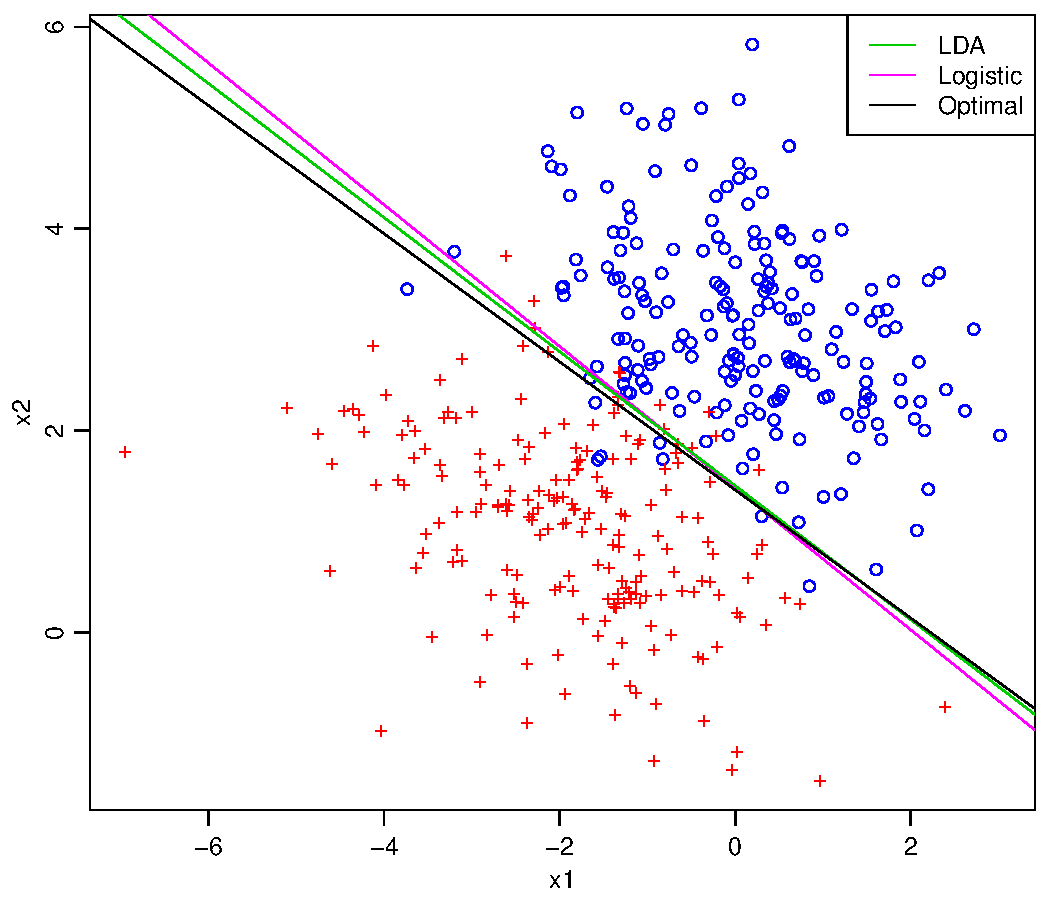
\includegraphics[scale=0.5]{./figures/ldaVsLogistic.pdf}
\end{center}
\caption{Decision boundaries for the two classes, each of size \Sexpr{N}, drawn from multigaussians with same covariance and different means.}
\label{fig:ldaVsLogistic}
\end{figure}
%
Although, the methods seem very similar, and in the toy example had almost equal performance, their can perform very different. LDA is based on some very special conditions, compared to logistic regression. In the derivation of Fisher's linear discriminant, it was clear that LDA can perform well outside the assumptions of normality, but logistic is still considered a more \textit{general} method. Therefore logistic regression is usually the preferred choice \cite[p.~128]{modstat}.
\\\colorbox{yellow}{Talk about how LDA can perform well for categorical variables, but logistic is better (modstat. p128}\\

